\documentclass[letterpaper,12pt]{article}
\usepackage[utf8]{inputenc}
\usepackage{fullpage}
\usepackage{courier}
\usepackage[margin=0.75in]{geometry}
\usepackage{listings}
\usepackage{color}
\usepackage{graphicx}
\usepackage[width=5in]{caption}
\usepackage{hyphenat}
\usepackage{hyperref}

% Format a sectionless paragraph
\newcommand*\unparagraph{
	\par
	\nopagebreak
	\vskip3.25ex plus1ex minus.2ex
	\noindent
}

% define extra colors
\definecolor{dkgreen}{rgb}{0,0.6,0}
\definecolor{purple}{RGB}{159,0,197}

% define the code listing format
\lstset{
	language=C++,
	basicstyle=\footnotesize\ttfamily,
	backgroundcolor=\color{white},
	showspaces=false,
	showstringspaces=false,
	frame=none,
	tabsize=3,
	keywordstyle=\color{purple},
	commentstyle=\color{dkgreen},
	stringstyle=\color{blue},
	escapeinside={\%*}{*)}
}

% efine the title/header
\title{\Large CS 3468\\Lab 3} 
\author{Jared Wallace}
\date{}

\begin{document}

\maketitle

\vspace{30mm}

\section*{Objectives}
\begin{enumerate}
\item Understand communication among sensors
\item Learn to read and use APIs (application programming interface) at
      \url{http://www.tinyos.net/tinyos-2.x/doc/nesdoc/micaz}
\end{enumerate}

\section*{Tasks}
\subsection*{Radio communication}


    Radio communication is used by sensors to exchange information. At least two parties are
    involved in communication: the sender and the receiver. Communication is done via
    the transmission of packets. Accordingly, a sensor that can send and receive via radio
    communication needs three components: \emph{AMSenderC} (in sender), \emph{AMReceiverC} (in receiver),
    and \emph{ActiveMessageC} (as radio control). TinyOS provides a number of interfaces
    to abstract the underlying communications services and a number of components that
    provide (implement) these interfaces. All of these interfaces and components use a
    common message buffer abstraction, called message\_t, which is implemented as a nesC
    struct (similar to a C struct).
    \begin{figure}[ht!]
        \centering
        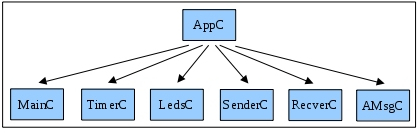
\includegraphics[width=4in]{tinyos-diagram.jpg}
       \caption*{The diagram shows a sensor application that can send and receive commands and also light LEDs according to commands. The application has seven components.}
    \end{figure}
    \begin{enumerate}
        \item System component MainC
        \item System component new TimerMilliC() as TimerC
        \item System component LedsC
        \item System component new AMSenderC(RADIOID) as SenderC
        \item System component new AMReceiverC(RADIOID) as RecverC
        \item System component ActiveMessageC as AmsgC
        \item Application component AppC
    \end{enumerate}
\subsection*{Reading and understanding an API}


    Now, open the API link \url{http://www.tinyos.net/tinyos-2.x/doc/nesdoc/micaz/}. Find the API
    documents of the first six system components.
    \begin{table}[htbp]
    \begin{center}
        \begin{tabular}{ |l|l|l| }
            \hline
            \textbf{Name} & \textbf{Description} & \textbf{Provides Interfaces} \\ \hline
            MainC & & \\ \hline
            TimerMilliC & & \\ \hline
            LedsC & & \\ \hline
            AMSenderC & & \\ \hline
            AMReceiverC & & \\ \hline
            ActiveMessageC & & \\ \hline
        \end{tabular}
    \end{center}
    \caption{Fill in this component table as your reference for further programming.}
    \end{table}
    \begin{table}[!hbp]
    \begin{center}
        \begin{tabular}{ |l|l|l|l| }
            \hline
            \textbf{Name} & \textbf{Components} & \textbf{Event functions} & \textbf{Description of events} \\ \hline
            & & & \\ \hline
            & & & \\ \hline
            & & & \\ \hline
            & & & \\ \hline
            & & & \\ \hline
            & & & \\ \hline
            & & & \\ \hline
            & & & \\ \hline
            & & & \\ \hline
        \end{tabular}
    \end{center}
    \caption{In this table, summarize all interfaces according to the component table. Use the API documents as reference.}
    \end{table}
\newpage
\subsection*{Read through and understand the source code of an application that communicates}


    Make sure you understand the following:
    \begin{itemize}
        \item How the seven components are wired through the interfaces
        \item When the events are called and how the events are handled
        \item How the AppC component makes use of system functions.
        \item How an AM message is defined.
    \end{itemize}

\subsection*{Compile and run the example application}
    \begin{itemize}
        \item Get two sensor IDs from the lab instructor. Use one for the sender and the other for the receiver. Modify Sender.h to include the receiver's ID.
        \item Modify the given code of the sender to send the following commands periodically and ligth the LEDs according to the following table.
        \item Modify the code of the receiver to receive the commands and light the LEDs according to the table.
        \item Use the assigned sensor IDs when loading the executable into sensors.
    \end{itemize}
    \begin{table}[htbp]
    \begin{center}
        \begin{tabular}{ |l|l|l|l| }
            \hline
            \textbf{Command} & \textbf{Yellow LED} & \textbf{Green LED} & \textbf{Red LED} \\ \hline
            0 & off & off & off \\ \hline
            2 & on & off & off \\ \hline
            4 & off & on & off \\ \hline
            6 & off & off & on \\ \hline
            8 & on & on & on \\ \hline
        \end{tabular}
    \end{center}
    \end{table}

\subsection*{Convert your app to be more reliable}


    The problem with the source code you have now is that it does not ensure reliable communication.
    Modify the source code to enforce reliable communication with per-packet acknowledgment.
    In another words, modify your code such that the transmission of a packet is successful
    only if the sender gets the acknowledgment from the receiver. Read over the APIs on the website to
    discover how to accomplish this.

    Next, design an experiment to check whether the radio communication is more reliable with
    the addition of the acknowledgment requirement. Collect data for analysis and use data
    as evidence for your findings.
\section*{Lab Report}
\begin{enumerate}
   \item Please demonstrate your program to the lab instructor and let him check your code at the end of the current lab project.
   \item Your project report is due at the beginning of the next lab.
   \item Grading criteria
      \begin{itemize}
         \item Demonstration, 15 percent
         \item Code, 15 percent
         \item Report, 70 percent
      \end{itemize}
\end{enumerate}
\section*{Report instructions}
Format:
\begin{enumerate}
   \item Include your name and ID in the first page
   \item Font size of at least 10pt
   \item Single spaced
   \item Maximum of 5 pages (I will take points off for exceeding this without any good reason)
   \item Please submit as PDF online, and turn in a hard copy
\end{enumerate}
Content:
\begin{enumerate}
   \item Introduction (10 percent of the report grade) Please summarize the task of this lab and what you have learned in the lab
   \item Implementation (30 percent of the report grade) Please describe in detail how your made your program. Show what components you used, how they are wired, and through what interfaces.
   \item Experiment (30 percent of the report grade) Please describe in detail what can be observed from your program and explain how said observed behavior is a result of your code (and not happy coincidence).
\end{enumerate}

% Comic at the bottom
\begin{figure}[ht!]
	\centering
	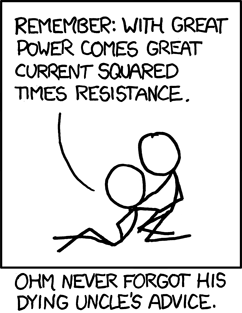
\includegraphics[width=3in]{ohm.png}
   \caption*{More generally, with great power comes great dEnergy/dt}
\end{figure}

\end{document}
